\Subhead{4.3.1}{Непрерывная генерация. Модуляция добротности. Синхронизация мод. Сверхкороткие импульсы}

В непрерывном режиме накачка и вывод энергии в среднем сбалансированы. Устойчивость интенсивности и инверсии проверяют скоростными уравнениями; постоянная мощность не означает отсутствия фазового шума.

При \emph{модуляции добротности} потери сначала велики: генерация подавлена, инверсия накапливается. Быстрое уменьшение потерь делает накопленное усиление надпороговым; поле истощает инверсию коротким мощным импульсом. Длительность переключения должна быть мала относительно накопления энергии, но реальный импульс определяется также временем обхода и ростом поля. Активный затвор задаётся извне, пассивный — насыщающимся поглотителем. Энергия импульса ограничена запасённым возбуждением и потерями, а не только скоростью затвора.

\emph{Синхронизация мод} фиксирует относительные фазы многих продольных частот $\omega_q=\omega_0+q\Omega_R$. Для $M$ равных фазированных амплитуд
\begin{equation}
 E(t)\propto\e^{-\ii\omega_0t}\sum_{q=0}^{M-1}\e^{-\ii q\Omega_Rt}
 =\e^{-\ii[\omega_0+(M-1)\Omega_R/2]t}
 \frac{\sin(M\Omega_Rt/2)}{\sin(\Omega_Rt/2)}.
\end{equation}
Возникает последовательность импульсов с периодом обхода $T_R=2\pi/\Omega_R$ и длительностью порядка $T_R/M\sim1/\Delta\nu$. Случайные фазы дают существенно меньший и нерегулярный максимум. Активная модуляция на FSR или насыщающийся поглотитель связывают моды; сам факт многомодовой генерации не означает синхронизацию. Q-модуляция меняет накопленную энергию, синхронизация мод — взаимные фазы; это разные способы импульсной работы.
\begin{center}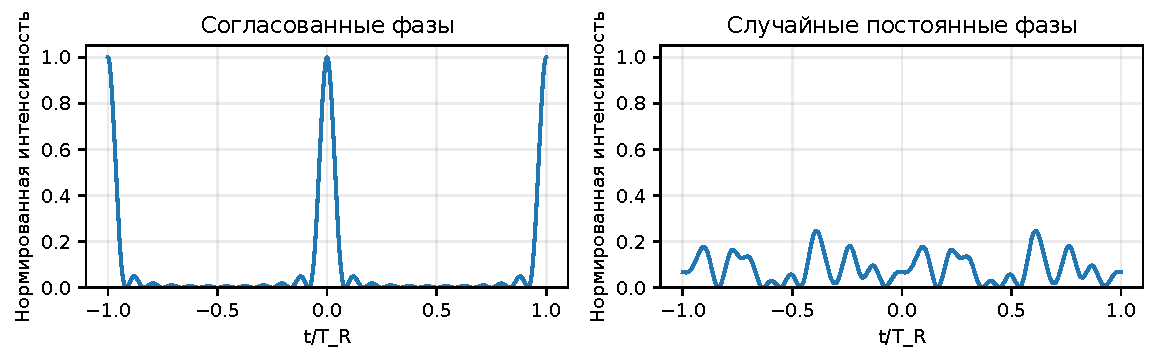
\includegraphics[width=0.8\linewidth]{figures/modelocking.pdf}\end{center}

